This spring-mass-pendulum-based example is presented to introduce \textit{bioptim}'s ability to use of external forces.
The goal was to maintain the position of a $\SI{1}{kg}$ mass hanging on a linear spring attached to the ground.
A $\SI{0.2}{m}$-long pendulum weighting $\SI{10}{kg}$ was attached to the mass and free to rotate in one dimension (Fig.~\ref{fig:Mass_Pendulum_Model}).
In addition to the spring force, the mass was actuated by a vertical external force (e.g., something pulling on it) while the pendulum rotation was passive.
The system therefore comprised two DoFs, the mass position ($q_m$) and the pendulum angle ($q_p$) and one control input, the vertical external force pulling on the mass ($f$). 
\begin{figure}[h!]
\centering
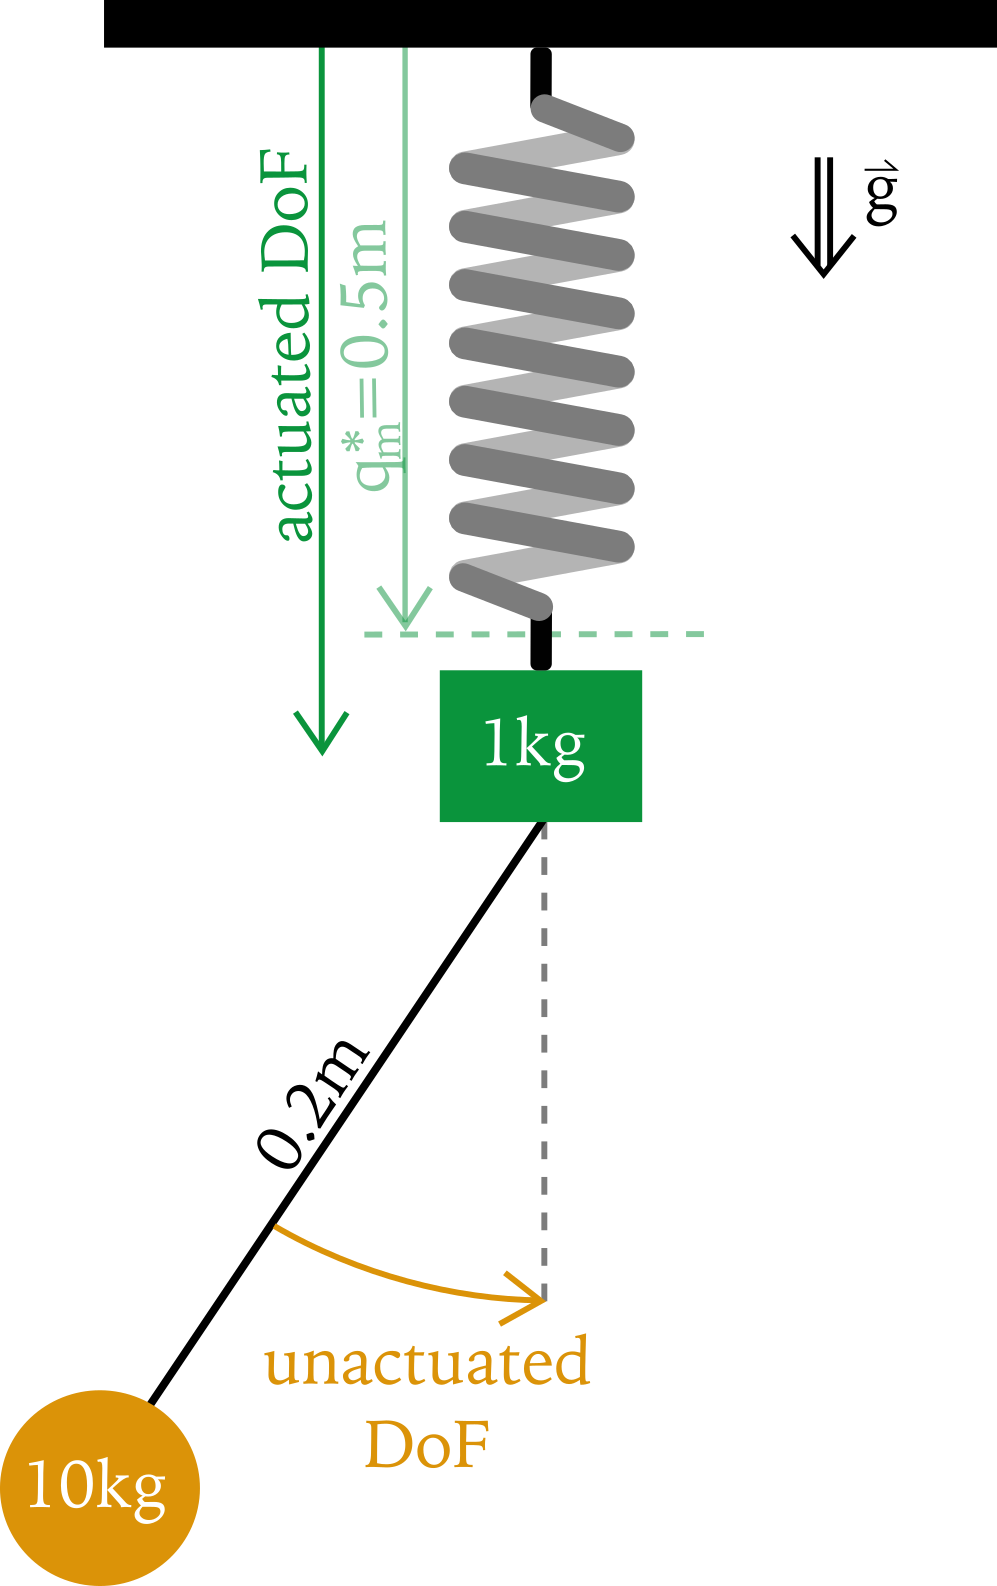
\includegraphics[width=0.35\columnwidth]{figures/Mass_Pendulum_Model.png}
\caption{Definition of the spring-mass-pendulum model.}
\label{fig:Mass_Pendulum_Model}
\end{figure}
The spring force $f_s$ was:
\[
\begin{aligned}
f_s = -k*q_m,
\end{aligned}
\addtag
\label{eq:f_ext}
\]
with k the spring stiffness constant.\\
The OCP was composed of two phases each lasting for $\SI{5}{s}$, with 50 shooting nodes.
In the first phase, no objective function was minimized and $f$ was constrained to $0$ letting the mass oscillating freely. 
Then, in the second phase, a cost function (Eq.\ref{eq:ocp_Pendulum}) was minimized, to enforce a specific position $q_m^*$ of the mass.
This objective function, exclusively composed of Lagrange terms, was formulated as follows:
\[
\mathcal{J} = \underbrace{\int_{T/2}^T (q_m - q_m^*)^2~dt}_{\mathtt{TRACK\_STATE}}  +~\omega_1 \underbrace{\int_{T/2}^T ~\tau^2~dt}_{\mathtt{MIN\_ TORQUE}},
\addtag
\label{eq:ocp_Pendulum}
\]

\noindent with $q_m$ and $q_m^* = -0.5m$ respectively the optimized and reference positions of the mass, $\omega_1 = 1\times 10^{-6}$, T the duration of the movement and $\tau$ the force control of the mass.
The first term of the objective function (Eq.~\ref{eq:ocp_Pendulum}) acts as a position controller for the mass.
The second was added for control regularization.


During the first phase, the mass is passively oscillating around its stationary position due to the spring force~\ref{fig:Mass_Pendulum_Fext_graphs}.
However, at the beginning of the second phase, when an additional external force is able to act on the mass, it stabilizes around the targeted position.
This example highlights the possibility of using optimal control to find activation patterns compensating for external passive forces (e.g., ortheses flexibility, contact surface deformation, interaction between two models, etc.).

\begin{figure*}[t!]
\centering
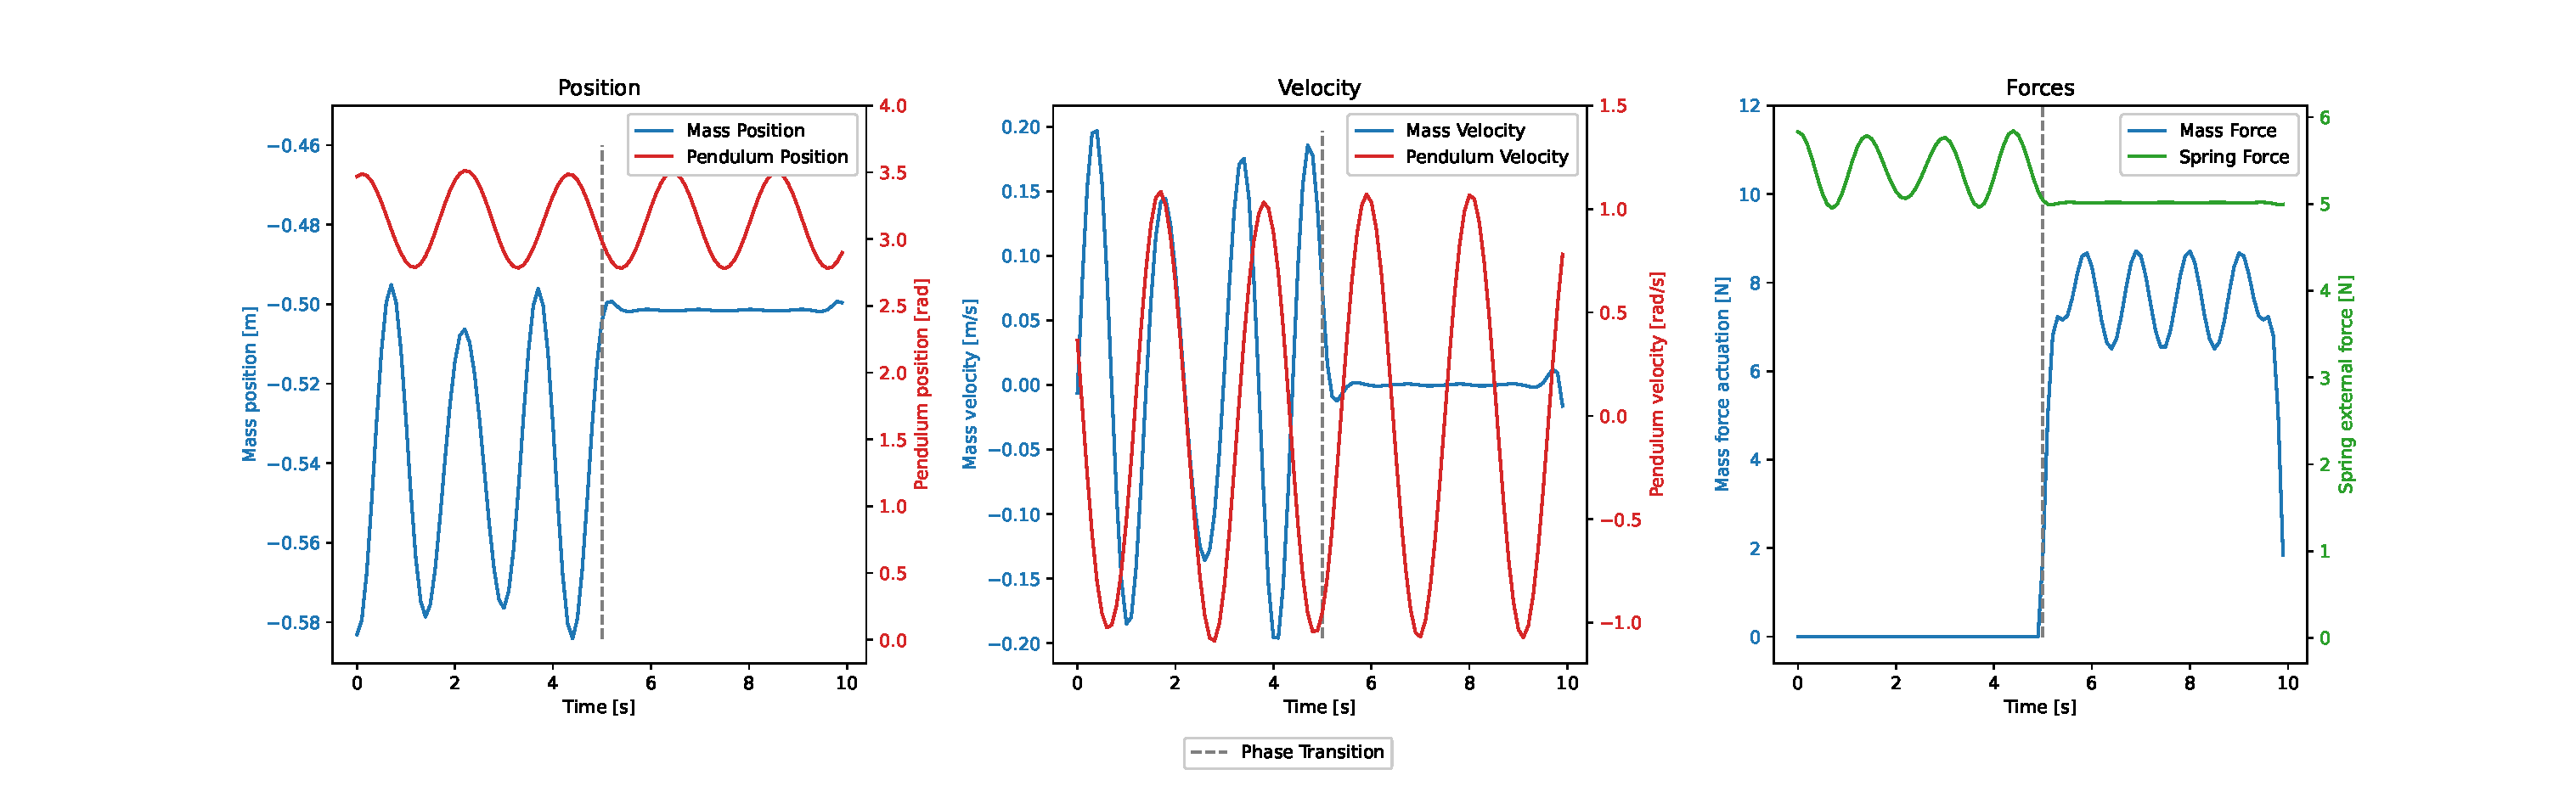
\includegraphics[width=\textwidth]{figures/Mass_Pendulum_Fext_2.eps}
\caption{Two-phases kinematics of the mass-pendulum-spring system. Gray dashed lines show the phase transition, blue lines are related to the mass (position velocity and external force acting on it), red lines are related to the pendulum (position and velocity) and the green line depicts the spring force.}
\label{fig:Mass_Pendulum_Fext_graphs}
\end{figure*}














